\chapter{Практические эксперименты и результаты}

В данной главе будут описаны практические исследования и полученные результаты нашего алгоритма. Сначала будет описано, на каких данных проводились результаты и как были устроены эксперименты, а после этого будут приведены диаграммы, описывающие сравнение нашего решения с существующими и подробное описание, объяснение и обсуждение результатов.

\section{Описание экспериментов}

Эксперименты были проведены на двух реальных датасетах: \textit{DBLP}~--- граф авторой статей, где ребро между авторами соответствует наличию у них общей статьи и \textit{Youtube}~--- граф пользователей социальной сети \textit{Youtube}, где ребро между пользователями означает обоюдную подписку.
Для экспериментов мы взяли $50$ случайных запросов без шума, $50$ запросов с шумом и $5$ запросов с абсолютным шумом, то есть с вершинами, которые практически никак между собой не связаны. Подробнее об этом дальше.

\begin{enumerate}
\item В качестве первого исследования мы взяли $50$ случайных запросов на графе, каждый из которых содержал вершины, довольно сильно коррелирующие между собой. В качестве запроса мы выбирали \textit{k-core} с достаточно большим $k$, а затем распределяли вершины-запросы в нем случайно, однако, следя за тем, чтобы они не были сильно далеко друг от друга, потому что иначе размеры подграфов будут довольно большими (это исследование рассматривается в статье Barbieri et al. \cite{Barbieri15}, у них размеры подграфов получаются примерно в $10$ раз больше, чем у нас. Это обусловлено только выбором вершин для запросов, наш выбор вершин больше соответствует актуальности нашей задачи). Как результат мы считали среднее результатов по этим $50$ экспериментам.

\item В качестве второго исследования мы брали $50$ случайных запросов на графе, каждый из которых содержал вершины, часть из которых довольно сильно коррелирует между собой, а часть (небольшая)~--- шум и плохо коррелирует с остальными вершинами. Фактически, первая часть вершин соответствует первому исследованию, а вторая часть вершин~--- просто добавленный шум. В качестве запроса мы выбирали \textit{k-core} с достаточно большим $k$ (то есть запрос, сгенерированный первым исследованием) с добавленными несколькими вершинами из \textit{k-core} с другими $k$, которые, соответственно, слабо коррелируют с остальными вершинами. Как результат мы считали среднее результатов по этим $50$ экспериментам.

\item В качестве третьего исследования, чтобы оценить поведение нашего алгоритма на практических абсолютно шумных запросах, мы выбираем несколько вершин из совсем разных \textit{k-core}, которые очень слабо или совсем не коррелируют между собой. Исследование показало, что на таких запросах наше решение строит достаточно большие по размеру итоговые подграфы, однако по максимуму отсеивая шум, что является довольно логичным эффектом в таком типе запросов.
\end{enumerate}

После каждого запуска алгоритм на вершинах-запросах мы также проводим валидацию ответа~--- что в полученном подграфе содержится большинство ($\max$($\frac{|Q|}{2}$, $|Q| \cdot \alpha - \epsilon$)) исходных вершин-запросов, где $\epsilon$~--- небольшое число, показывающее, что после шага $2$ мы также могли удалить несколько слабо связанных вершин на третьей фазе, которое для наших исследований мы брали равным $4$.

\section{Результаты экспериментов}

 Здесь мы приведем результаты экспериментов, сравнивающие предложенный алгоритм, алгоритм Faloutsos \& Tong \cite{Faloutsos06}, Gionis et al. \cite{Gionis15} и Barbieri et al. \cite{Barbieri15}. Для визуализации результатов будут приведены диаграммы с краткими описаниями. Для каждого из двух датасетов будет приведено $6$ диаграм, сравнивающие плотности и размеры полученных рассмотренными алгоритмам подграфов, а также время работы этих алгоритмов (без учета времени построения индекса). Диаграммы строятся для $2$ типов запросов~--- без шума и с ним соответственно. В каждой диаграмме горизонтальная ось соответствует различным размерам выбранных запросов $|Q|$ (рассмотренные значения $|Q|$: $1$, $2$, $3$, $4$, $8$, $16$ и $32$), а вертикальная ось соответствует плотности полученного подграфа, его размеру или же времени работы алгоритма.

\subsection{Датасет DBLP}

В датасете \textit{DBLP} $317080$ вершин и $1049866$ ребер. Датасет состоит из авторов различных статей, а ребро между авторами соответствует наличию у них общей статьи.

\subsubsection{Запросы без шума. Плотность подграфа}

%\begin{figure}[!h]
%\caption{Запросы без шума. Плотность подграфа.}\label{dblp-density}
  \begin{center}
    \makebox[\textwidth]{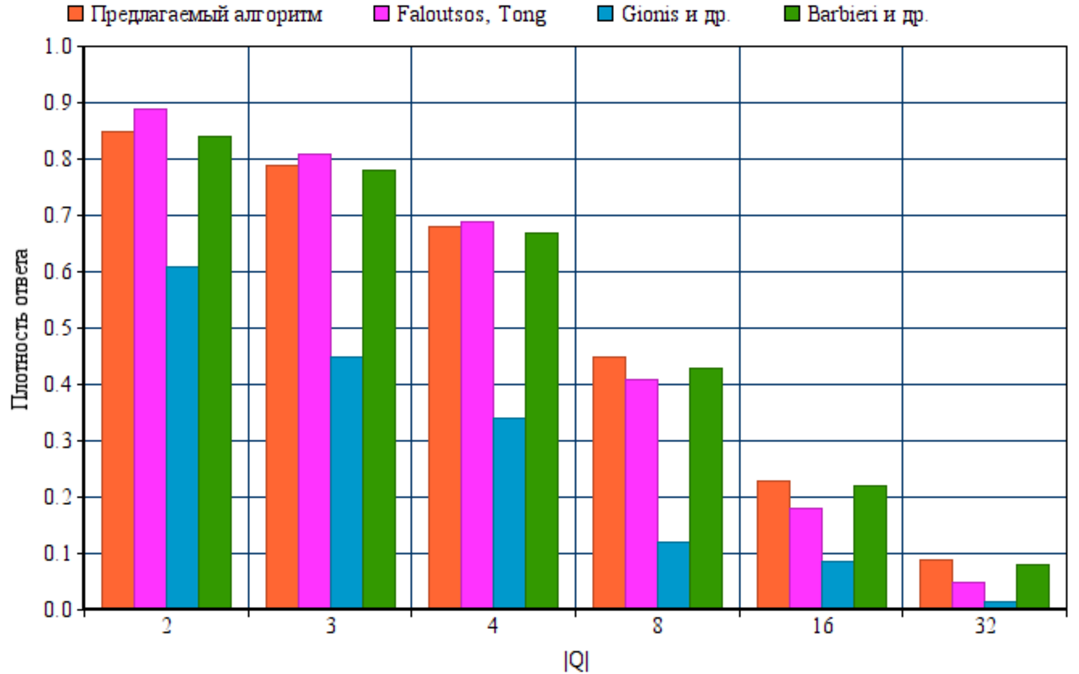
\includegraphics[scale=0.4]{pictures/results-dblp-density.png}}
  \end{center}
%\end{figure}

Как видно из диаграммы, на случайных запросах без шума плотность нашего полученного подграфа меньше, хоть и совсем немного, плотности подграфа, полученного статьей Barbieri et al. \cite{Barbieri15}, а значит наш ответ оптимальнее. Также плотность нашего подграфа в среднем больше плотности Faloutsos \& Tong \cite{Faloutsos06} (она совсем немного меньше при небольших значениях $|Q|$ из-за структуры их алгоритма, однако при б\'{о}льших значениях $|Q|$ мы начинаем сильно выигрывать по плотности) и намного больше плотности Gionis et al. \cite{Gionis15}, потому что статья этих авторов, хоть и умеет решать поставленную нами задачу, плотность полученного подграфа~--- не ее первоочередная цель.

\subsubsection{Запросы без шума. Размер подграфа}

%\begin{figure}[!h]
%\caption{Запросы без шума. Размер подграфа.}\label{dblp-size}
  \begin{center}
    \makebox[\textwidth]{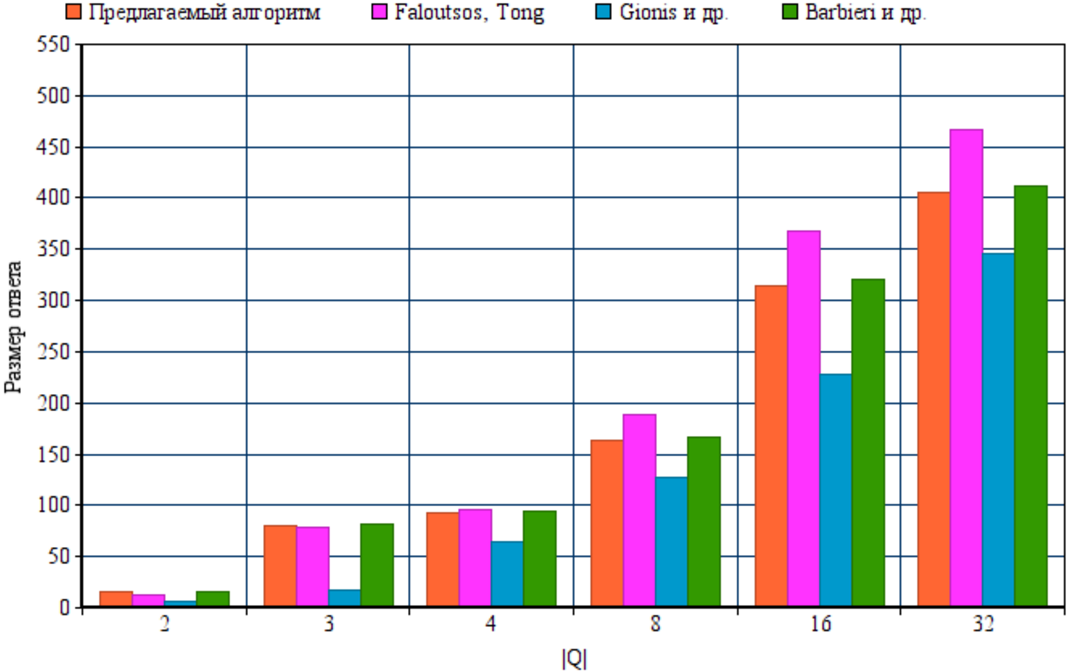
\includegraphics[scale=0.4]{pictures/results-dblp-size.png}}
  \end{center}
%\end{figure}

Как видно из диаграммы, на случайных запросах без шума размер нашего полученного подграфа также немного, но меньше размера подграфа, полученного статьей Barbieri et al. \cite{Barbieri15}, из чего становится логичным, откуда получено улучшение по плотности. Размер нашего подграфа в среднем меньше размера подграфа Faloutsos \& Tong \cite{Faloutsos06}, хоть и для небольших $|Q|$ их решение работает лучше из-за его построения, но меньше размера Gionis et al. \cite{Gionis15}, потому что в этом как раз и состоит предназначение их статьи.

\subsubsection{Запросы без шума. Время работы}

%\begin{figure}[!h]
%\caption{Запросы без шума. Время работы.}\label{dblp-time}
  \begin{center}
    \makebox[\textwidth]{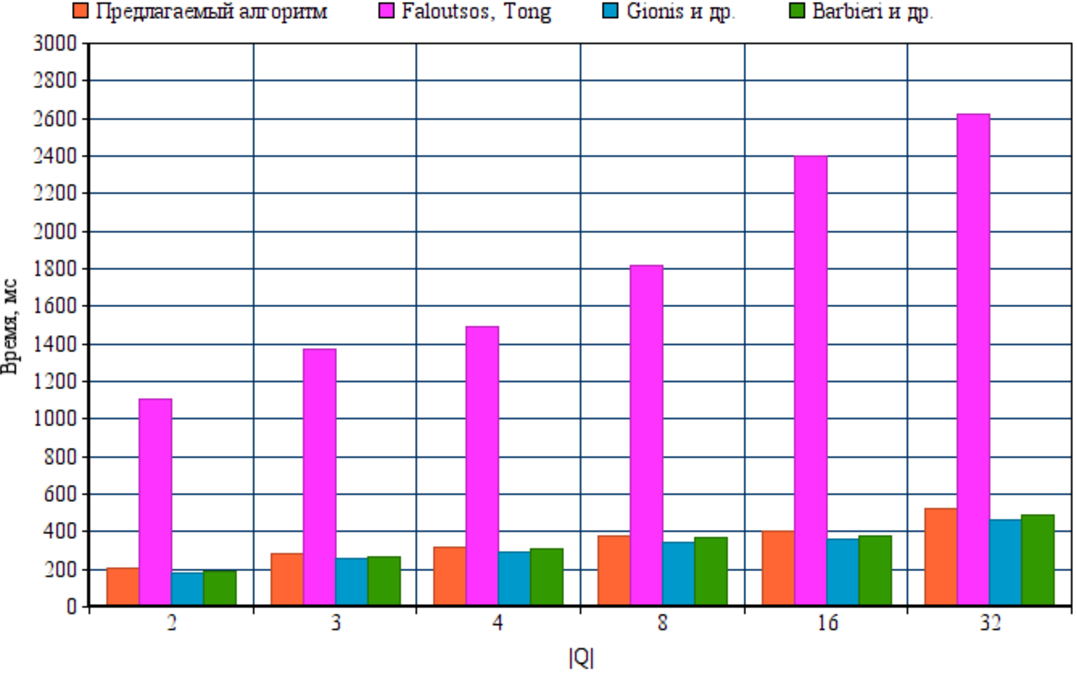
\includegraphics[scale=0.4]{pictures/results-dblp-time.png}}
  \end{center}
%\end{figure}

Как видно из диаграммы, по времени мы немного проигрываем статье Barbieri et al. \cite{Barbieri15}, однако этот проигрыш совсем незначительный. Faloutsos \& Tong \cite{Faloutsos06} работают сильно дольше нас, а Gionis et al. \cite{Gionis15} быстрее, но это не является нашим минусом, посколько плотность подграфов, получаемых этих алгоритмом намного меньше нашей.

\subsubsection{Запросы c шумом. Плотность подграфа}

%\begin{figure}[!h]
%\caption{Запросы c шумом. Плотность подграфа.}\label{dblp-density-noise}
  \begin{center}
    \makebox[\textwidth]{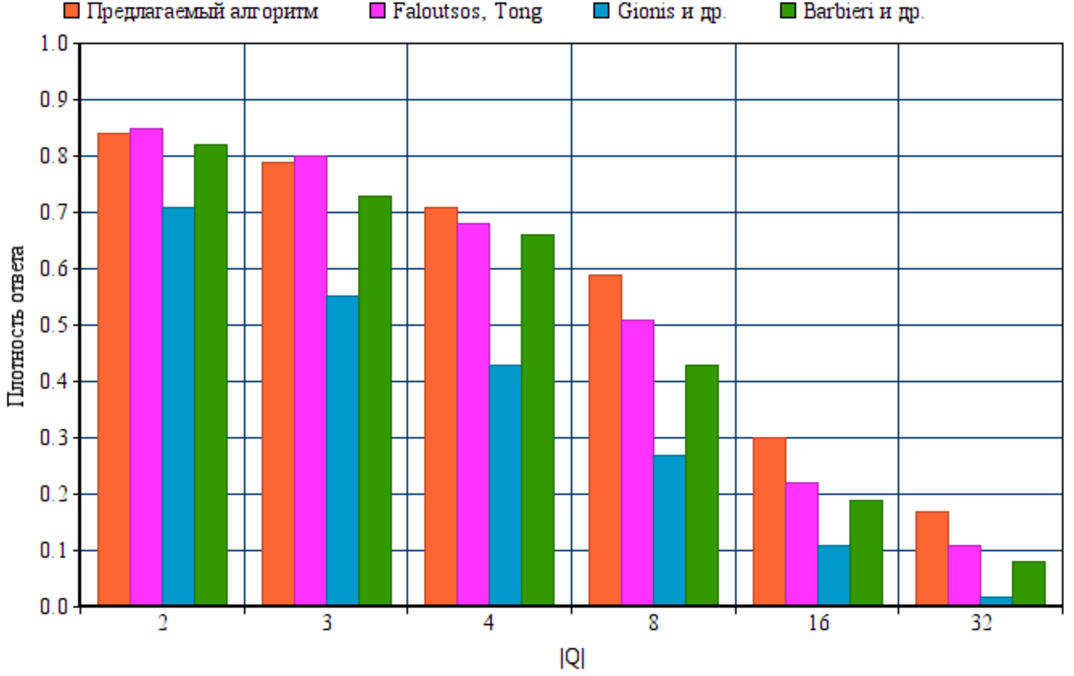
\includegraphics[scale=0.4]{pictures/results-dblp-density-noise.png}}
  \end{center}
%\end{figure}

Если в запросе появляется шум, наш алгоритм начинает работать сильно оптимальней. Это видно из представленной выше диаграммы: при небольших значениях $|Q|$ наш выигрыш мал, что логично, потому что шума в таких запросах практически быть не может, однако, при б\'{о}льших значениях $|Q|$ мы начинаем сильно выигрывать по плотности и размеру итогового подграфа (см. следующую диаграму). 

\subsubsection{Запросы с шумом. Размер подграфа}

%\begin{figure}[!h]
%\caption{Запросы c шумом. Размер подграфа.}\label{dblp-size-noise}
  \begin{center}
    \makebox[\textwidth]{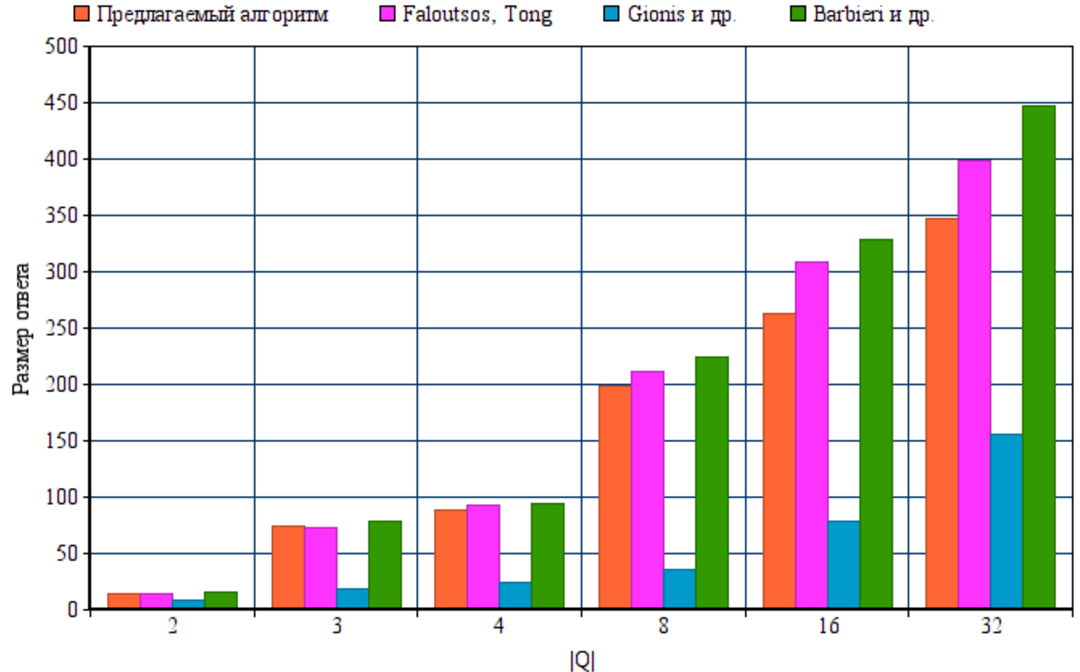
\includegraphics[scale=0.4]{pictures/results-dblp-size-noise.png}}
  \end{center}
%\end{figure}

Как можно видеть из диаграммы, при наличии шума, размер нашего подграфа также меньше размера подграфов остальных решений (кроме Gionis et al. \cite{Gionis15}, но так и должно быть), что объясняет выигрыш по плотности в предыдущей диаграмме.

\subsubsection{Запросы с шумом. Время работы}

%\begin{figure}[!h]
%\caption{Запросы c шумом. Время работы.}\label{dblp-time-noise}
  \begin{center}
    \makebox[\textwidth]{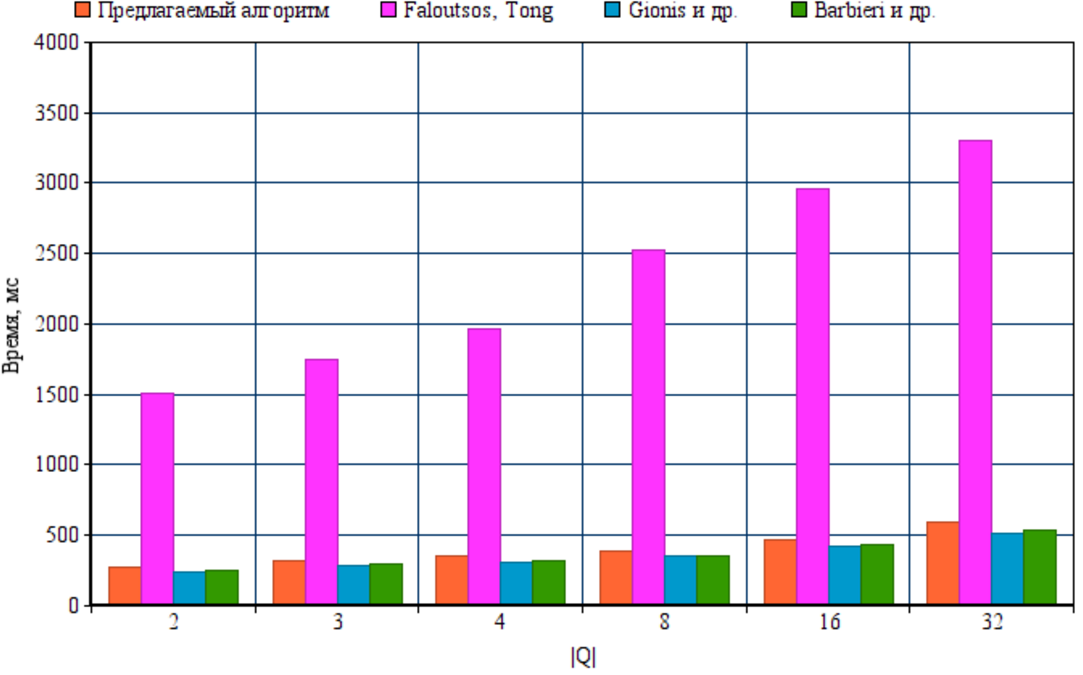
\includegraphics[scale=0.4]{pictures/results-dblp-time-noise.png}}
  \end{center}
%\end{figure}

Время работы предложенного алгоритма на запросах с шумом также немного больше времени работы Barbieri et al. \cite{Barbieri15}, однако проигрыш по времени совсем незначительный по сравнению с улучшением результатов плотности и размера.

\subsection{Датасет Youtube}

В датасете \textit{Youtube} $1134890$ вершин и $2987624$ ребер. Датасет состоит из пользователей социальной сети \textit{Youtube}, ребро между пользователями существует, если они друг у друга в друзьях.

Результаты практически совпадают с результатами на датасете \textit{DBLP}, за исключением глобальных изменений во времени работы из-за размера датасета, поэтому комментарии к диаграммам будут приведены только в случае необходимости.

\subsubsection{Запросы без шума. Плотность подграфа}

%\begin{figure}[!h]
%\caption{Запросы без шума. Плотность подграфа.}\label{youtube-density}
  \begin{center}
    \makebox[\textwidth]{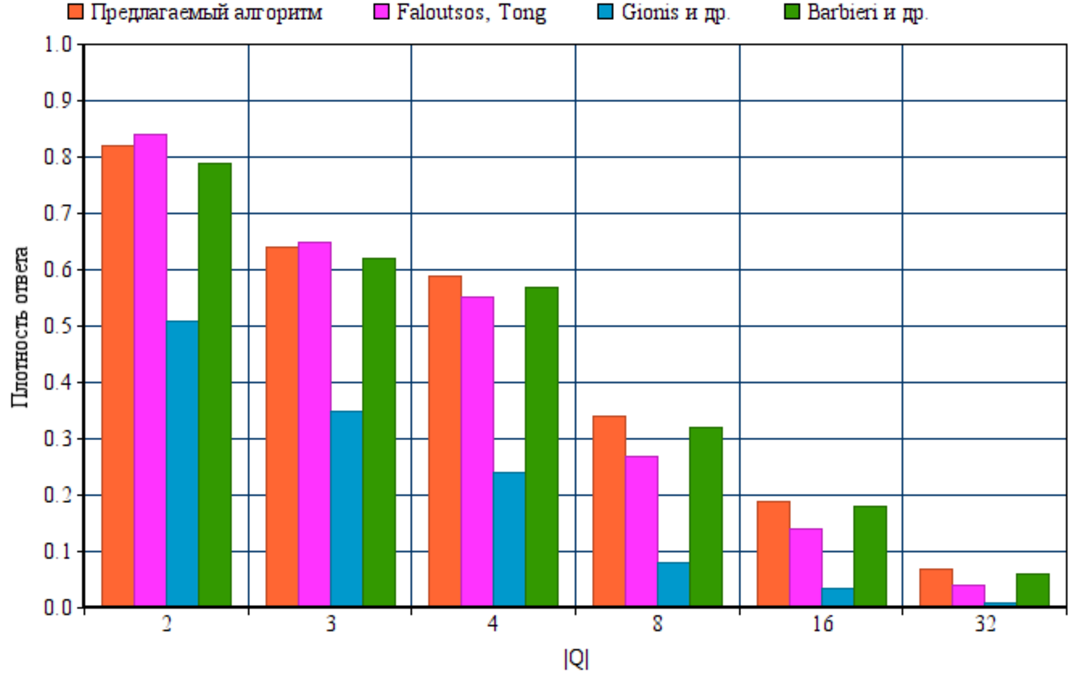
\includegraphics[scale=0.4]{pictures/results-youtube-density.png}}
  \end{center}
%\end{figure}

\subsubsection{Запросы без шума. Размер подграфа}

%\begin{figure}[!h]
%\caption{Запросы без шума. Размер подграфа.}\label{youtube-size}
  \begin{center}
    \makebox[\textwidth]{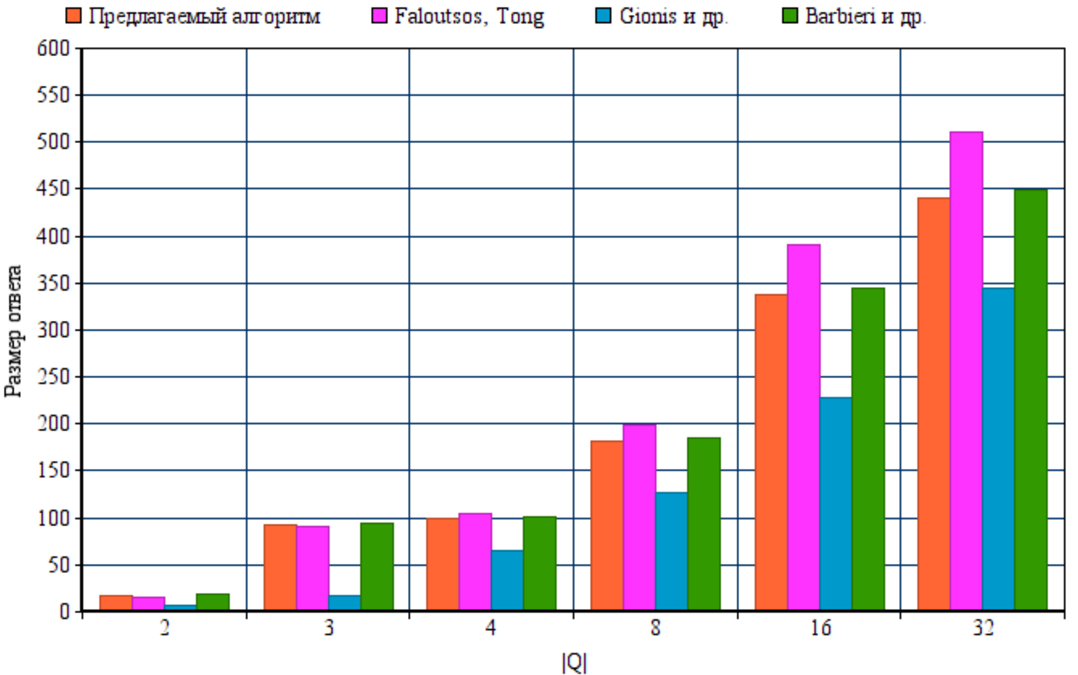
\includegraphics[scale=0.4]{pictures/results-youtube-size.png}}
  \end{center}
%\end{figure}
%\FloatBarrier

\subsubsection{Запросы без шума. Время работы}

%\begin{figure}[!h]
%\caption{Запросы без шума. Время работы.}\label{youtube-time}
  \begin{center}
    \makebox[\textwidth]{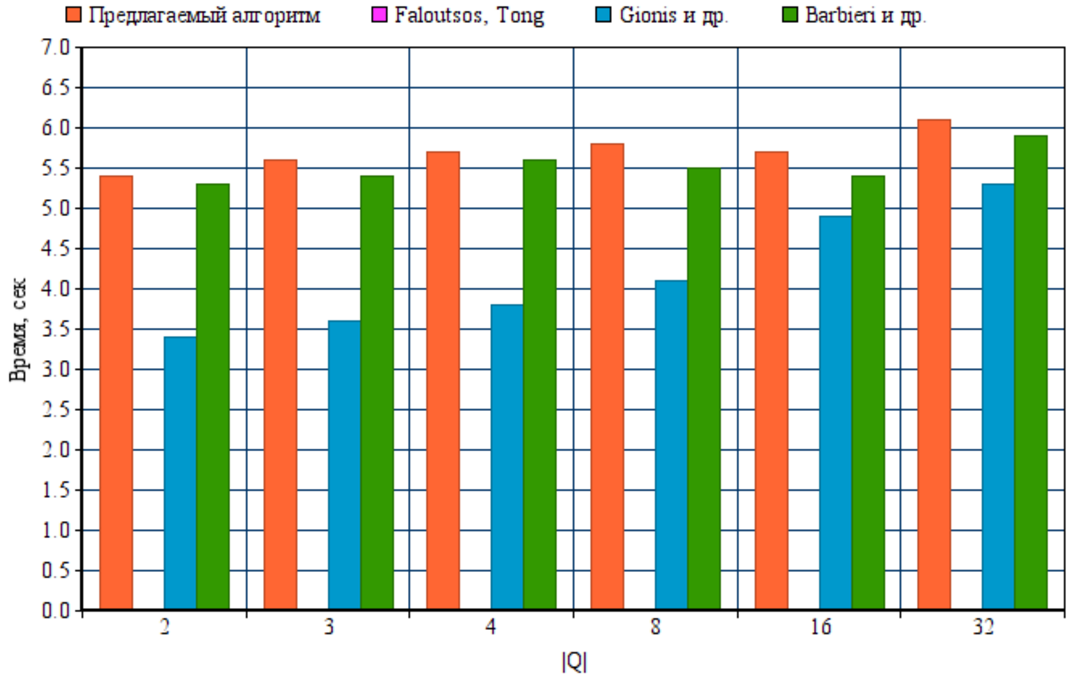
\includegraphics[scale=0.4]{pictures/results-youtube-time.png}}
  \end{center}
%\end{figure}

Здесь стоит отметить, что алгоритм Faloutsos \& Tong \cite{Faloutsos06} работает слишком долго и чтобы не нарушать визуальность относительности времени работы остальных алгоритмов, этот алгоритм в диаграмме опущен. Также стоит отметить, что время работы изменяется в секундах в отличие от предыдущего датасета из-за значительной разницы в их размерах.

\subsubsection{Запросы c шумом. Плотность подграфа}

%\begin{figure}[!h]
%\caption{Запросы с шумом. Плотность подграфа.}\label{youtube-density-noise}
  \begin{center}
    \makebox[\textwidth]{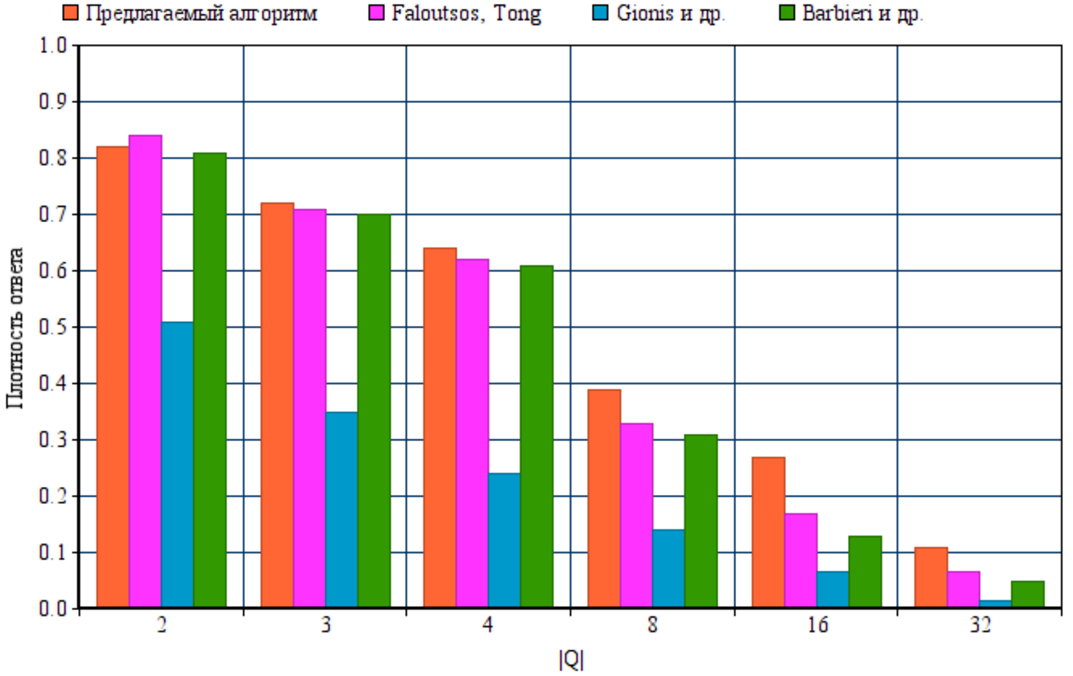
\includegraphics[scale=0.4]{pictures/results-youtube-density-noise.png}}
  \end{center}
%\end{figure}

\subsubsection{Запросы с шумом. Размер подграфа}

%\begin{figure}[!h]
%\caption{Запросы с шумом. Размер подграфа.}\label{youtube-size-noise}
  \begin{center}
    \makebox[\textwidth]{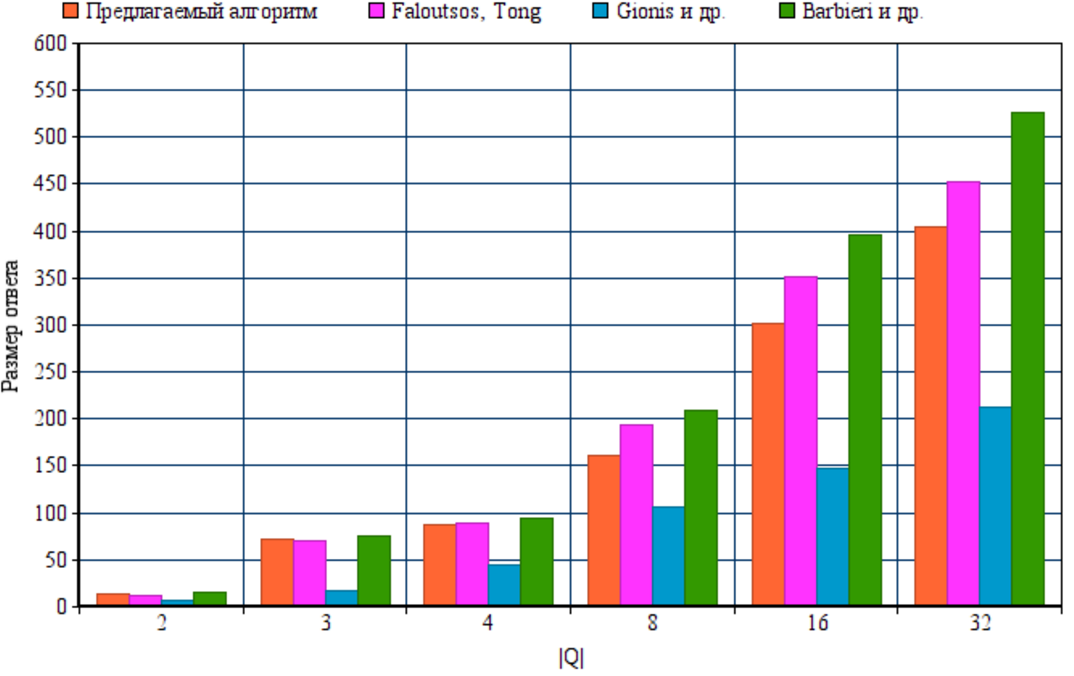
\includegraphics[scale=0.4]{pictures/results-youtube-size-noise.png}}
  \end{center}
%\end{figure}
%\FloatBarrier

\subsubsection{Запросы с шумом. Время работы}

%\begin{figure}[!h]
%\caption{Запросы с шумом. Время работы.}\label{youtube-time-noise}
  \begin{center}
    \makebox[\textwidth]{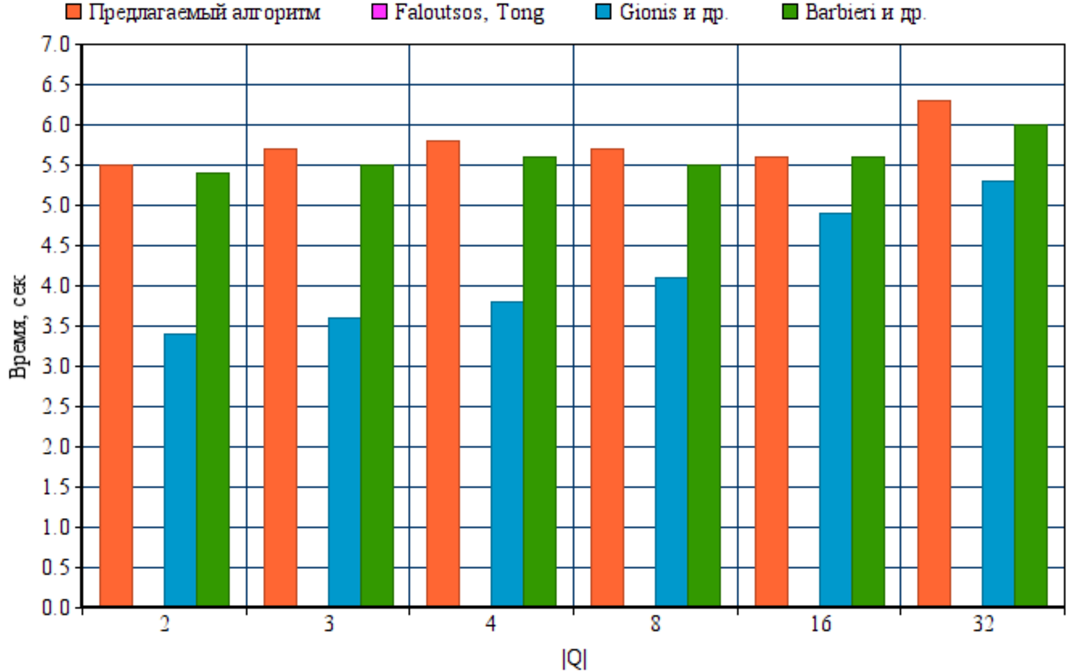
\includegraphics[scale=0.4]{pictures/results-youtube-time-noise.png}}
  \end{center}
%\end{figure}
%\FloatBarrier

Здесь время работы алгоритма Faloutsos \& Tong \cite{Faloutsos06} не указано по той же причине, что и в диаграмме с запросами без шума.

\subsection{Итоговые результаты}

Соберем результаты приведенных диаграмм в таблицах~\ref{results-dblp} и ~\ref{results-youtube}:

В таблицах указано, как соотносится наше решение с тремя рассмотренными. В каждой ячейке через записаны средний результат и максимальный выигрыш соответственно. Так, например, $18.1\%/54.6\%$ в плотности с шумом означает, что мы в среднем выиграли $18.1\%$ по плотности, а максимум по всем экспериментам~--- $54.6\%$. В размере и времени же $-4.7\%/-14.6\%$ означает, что наш размер на $4.7\%$ меньше в среднем и на $14.6\%$ меньше в максимальном случае соответственно.

\begin{table}[!h]
\centering
\caption{DBLP - сравнение предлагаемого алгоритма с существующими решениями}\label{results-dblp}
  \begin{tabular}{| l | l | l | p{4cm} |}
  \hline
  -- & Faloutsos \& Tong & Gionis et al. & Barbieri et al. \\\hline
  Плотность       & +18.2\% / +80.0\% & +200.6\% / +542.9\% & 4.2\%   / +12.5\%  \\\hline
  Размер          & -4.5\%  / -14.4\% & +97.4\%  / +17.7\%  & -2.9\%  / -6.25\%  \\\hline
  Время           & -80.3\% / -83.3\% & +11.7\%  / +7.7\%   & +5.2\%  / +2.7\%   \\\hline
  Плотность (шум) & +18.1\% / +54.6\% & +210.4\% / +844.4\% & +37.6\% / +112.5\% \\\hline
  Размер (шум)    & -4.7\%  / -14.6\% & +247.9\% / +87.5\%  & -11.6\% / -22.4\%  \\\hline
  Время (шум)     & -82.8\% / -84.6\% & +12.1\%  / +10.3\%  & +8.4\%  / +6.6\%   \\\hline
  \end{tabular}
\end{table}
\FloatBarrier

\begin{table}[!h]
\centering
\caption{Youtube - сравнение предлагаемого алгоритма с существующими решениями}\label{results-youtube}
  \begin{tabular}{| l | l | l | p{3.8cm} |}
  \hline
  -- & Faloutsos \& Tong & Gionis et al. & Barbieri et al. \\\hline
  Плотность       & +23.3\%  / +75.0\%  & +305.4\% / +775.0\% & +6.5\%  / +16.7\%  \\\hline
  Размер          & -4.6\%   / -13.7\%  & +123.3\% / +27.9\%  & -2.6\%  / -5.3\%   \\\hline
  Время           & -320.8\% / -325.1\% & +39.6\%  / +15.1\%  & +3.6\%  / +1.8\%   \\\hline
  Плотность (шум) & +24.7\%  / +69.2\%  & +252.1\% / +685.7\% & +45.3\% / +129.2\% \\\hline
  Размер (шум)    & -4.3\%   / -17.0\%  & +223.3\% / +27.8\%  & -14.8\% / -23.7\%  \\\hline
  Время (шум)     & -323.4\% / -331.1\% & +40.8\%  / +14.2\%  & +2.9\%  / +0.0\%   \\\hline
  \end{tabular}
\end{table}
\FloatBarrier

Также нас интересует еще одна вещь~--- не может ли быть так, что на запросе без шума мы выкинем лишние вершины? Проведенные эксперименты показали, что на самом деле такое возможно, и наш алгоритм на запросах без шума может выкинуть несколько вершин, решив, что это шум. Однако, так как на самом деле шума нету и вершины довольно плотно связаны, таких вершин будет мало или вообще не будет. Результаты показали, что мы выкидываем не больше $2-3$ вершин из $Q$ (при $|Q| = 32$), что вполне нормально. Напомним, что этого можно избежать, воспользовавшись обратной совместимостью, описанной в конце главы $2$~--- мы можем немного изменить наш алгоритм, чтобы он решал исходную задачу SCP, тогда все вершины-запросы будут включены в ответ.

\chapterconclusion

В главе были описаны методы проведения экспериментов на двух датасетах \textit{DBLP} и \textit{Youtube}, полученные результаты показывают, что наш алгоритм на случайных запросах с коррелирующими вершинами работает даже чуть лучше предыдущего решения \cite{Barbieri15}, однако немного проигрывая ему по времени. Однако, на запросах, содержащих шум, наш алгоритм работает намного лучше существующих и выдает подграфы по плотности и размеру сильно улучшающие имеющиеся решения.
